\documentclass{article}

\usepackage{natbib}
\usepackage[bookmarks=false]{hyperref}
\usepackage{mathtools}
\usepackage{amssymb,amsmath}
\usepackage{textcomp}
\usepackage{url}
\usepackage{caption}
\usepackage{subcaption}
\usepackage{tabulary}
\usepackage{setspace}

\usepackage{balance}
\usepackage{flafter}
\usepackage[linesnumbered,ruled]{algorithm2e}
\usepackage{algpseudocode}
\usepackage{amsmath}
\usepackage{varwidth}
\SetKwInOut{Input}{Input}
\SetKwInOut{Output}{Output}
\usepackage{color}
\newcommand\todo[1]{\textcolor{blue}{(todo : #1)}}
\DontPrintSemicolon
\usepackage[utf8]{inputenc}


\allowdisplaybreaks
\hyphenation{op-tical net-works semi-conduc-tor}

\doublespacing
\begin{document}

\title{Knowledge Distillation As A Possible Solution For Domain Transfer  \\
\large{A Dissertation Proposal Submitted In Partial Fulfillment Of PhD Comprehensive Exam \\
}}
\author{Mithun Paul\\}



\maketitle

\tableofcontents

\section{Problem Statement}

The task of natural language inference is considered to be an integral part of natural language understanding. In this task, which can be seen as a particular instance of recognizing textual entailment \citep*{fyodorov2000natural,condoravdi2003entailment,bos2005recognising,maccartney2009extended,dagan2013recognizing}, a model is asked to classify if a given sentence (premise) \textit{entails}, \textit{contradicts} or is \textit{neutral} given a second sentence (hypothesis). Several data sets have been created which have enabled the advancement of natural language inference (and fact verification) like SNLI \citep*{bowman2015large} MNLI \citep*{williams2017broad}, FEVER \citep*{thorne2018fever}, and FNC \citep*{pomerleau2017fake}. The state-of-the-art  performance in many of these datasets domains have been achieved by many neural network methods \citep*{kim2018semantic}.

However it is known that these datasets are not devoid of biases (subtle statistical patterns in a dataset, which could have been introduced either due to the methodology of data collection or due to an inherent social bias). For example, \citep*{gururangan2018annotation} and \citep*{poliak2018hypothesis} show that biases were introduced into the MNLI dataset by certain language creation choices made by the crowd workers. 

These biases can be readily exploited by neural networks and thus have influence on performance.  As an example, \citep*{gururangan2018annotation} demonstrate that many state of the art methods in natural language inference could still achieve reasonable accuracies when trained with the hypothesis alone. This tendency of neural networks to inadvertently exploit such dataset artifacts is likely worsened by the fact that currently the success of natural language processing approaches is almost exclusively measured by empirical performance on benchmark datasets. While this emphasis on performance has facilitated the development of practical solutions, they may lack guidance as they are often not motivated by more general linguistic principles or human intuition. This makes it difficult to accurately judge the degree to which these methods actually extract reasonable representations, correlate with  human intuition or understand the underlying semantics~\citep*{dagan2013recognizing}.



While doing  early experiments in the fact verification space, I observed that out of all the statements containing the phrase ``American Author,'' 91\% of them belonged to one class label. I suspected that the state-of-the-art neural network methods depended heavily on these lexical information. Such information could be meaningful in the literature news domain, but transfers poorly to other domains such as science or entertainment.  


Hence as part of my research, I aim to understand and estimate the importance that a neural network assigns to various aspects of the data while learning and making predictions and also to propose solutions to mitigate this dependency.


In this context, the aims of my research are:


\begin{itemize}

\item I investigate the attention weights a state of the art RTE method~\cite{parikh2016decomposable} assigns to input tokens in the RTE component of fact verification systems, and confirm that most of the weight is assigned to POS tags of nouns (e.g., NN, NNP etc.) or their phrases, which verified my ``American Author" observation stated above.
\item  To verify that these lexicalized models transfer poorly, I implement a domain transfer experiment where a RTE component is trained on the FEVER data, and tested on the Fake News Challenge (FNC) \citep{pomerleau2017fake} dataset. As expected, even though this method achieves high accuracy when evaluated in the same domain, the performance in the target domain is poor, marginally above chance.

\item  To mitigate this dependence on lexicalized information, I experiment with several strategies for masking out names by replacing them with their semantic category, coupled with a unique identifier to mark that the same or new entities are referenced between claim and evidence. The results show that, while the performance on the FEVER dataset remains at par with that of the model trained on lexicalized data, it improves significantly when tested in the FNC dataset. Thus my experiments demonstrate that my strategy is successful in mitigating the dependency on lexical information.

\item I propose a framework based on fact distillation to train neural network models which can learn the underlying semantics of a given dataset and hence can be used to transfer learning across domains.
\end{itemize}

\section{Preliminary Work}


In this section I describe several preliminary experiments I conduct to verify that models trained on lexicalized data transfer poorly across domains. In particular I investigate the attention weights a state of the art recognizing textual entailment method~\citep*{parikh2016decomposable} assigns to input tokens in the recognizing textual entailment component of fact verification systems, and confirm that most of the weight is assigned to POS tags of nouns (e.g., neural network, NNP etc.) or their phrases, which verify my ``American Author" observation stated above. Further I also show results from a few proposed solutions which control for unnecessary lexicalization enabling data transfer across domains.



\subsection{Experiment Set-Up}
 
To verify that models trained on lexicalized data transfer poorly, I implement a domain transfer experiment where a state-of-the-art recognizing textual entailment model is trained on one dataset (FEVER \citep*{thorne2018fever}) and tested on another dataset (Fake News Challenge \citep*{pomerleau2017fake}). In particular, the neural network method I use is the Decomposable Attention (decomposable attention) \citep*{parikh2016decomposable}, which consistently achieves near state-of-the-art performance on recognizing textual entailment tasks \footnote{This experiment was initially setup during the 2018 FEVER shared task which had provided Decomposable Attention as a strong baseline. At the completion of the shared task, most of the winning teams used another model \citep*{chen2016enhanced}. However, the aim of my work is not to outperform the state of the art performance, but rather to generalize to new domains without retraining.}.  I use the AllenNLP \footnote{\url{https://github.com/allenai/allennlp}}
implementation of decomposable attention, which was provided by the FEVER task organizers. To investigate DA's reliance on lexical information, I first examine its word-level attention weights (Section \ref{attention_analysis}). 
Informed by these results, I propose several methods to mask the lexicalized data (Section \ref{masking_techniques}), and evaluate them in in-domain and  out-of-domain settings (Section \ref{sec:results}).




\begin{table*}[t]
    \centering
    \footnotesize
    \begin{tabular}{ccccc}
        Dataset & Support & Refute & Discuss & Unrelated \\
        \hline
        FNC    & 5,581 & 1,537  & 13,373 & 54,894 \\
        FEVER  &  86,701 & 36,441  & \multicolumn{2}{c}{42,305 (\textit{NEI})} \\  
    \end{tabular}
    \caption{Label distribution for the FEVER and FNC datasets.  I consider the \textit{agree} and \textit{disagree} FNC labels as equivalent to the \textit{support} and \textit{refute} labels in FEVER. The FNC \textit{not enough info (NEI)} label is listed below the more fine-grained \textit{discuss} and \textit{unrelated} FEVER labels.  }
    \label{tab:data}
\end{table*}

\subsection{Datasets}
For analyzing the effects of various delexicalization operations I chose four  popular datasets in natural language inference (NLI): Multi-genre NLI (MNLI) dataset \cite{williams2017broad}, Fact Extraction and Verification  (FEVER) dataset~\cite{thorne2018fever}, the Fake News Challenge (FNC ) dataset \cite{pomerleau2017fake}, and the Medical NLI (MedNLI) dataset \cite{romanov2018lessons}. In MNLI the trained models were tested on both of the validation partitions, the matched partition (which serves as the in-domain partition) and mismatched (the out-of-domain) partition.

Here I take one of the datasets (FEVER \citep*{thorne2018fever}) as an example and trace various issues that were encountered in the data pre-processing phase used to normalize labels and format across all these datasets.


{\flushleft{\bf Fact Extraction and Verification (FEVER):}} The FEVER \citep*{thorne2018fever} dataset consists of 145,449 training data points, each of which has a claim and a set of evidences retrieved from Wikipedia using a baseline information retrieval (IR) module.
The FEVER claim-evidence pairs were assigned labels from three classes: \textit{supports}, \textit{refutes}, and \textit{not enough info (NEI)} . Even though the partition of the FEVER dataset that was used in the final shared task competition was released publicly, the gold test labels were not. Hence I used the development portion (19,998 data points) instead as my test partition. I created my own development partition by randomly dividing the training partition into 80\% for training (119,197 data points) and 20\% (26,252 data points) for development.  The evidence for data points that had the gold label of \textit{not enough info} can be retrieved (using a task-provided IR component) either by finding the nearest neighbor to the claim or randomly \citep*{thorne2018fever}. 


\subsubsection{Cross-domain Labels}
\label{sec:crossdomain}


In order to evaluate models in a cross-domain setting, I modified the label space of the source domain to match that of the target domain. This  also allows us to evaluate using the official scoring measures of the target domain. In particular, when training on FEVER and testing on FNC, the data points in FEVER that belong to the class \textit{supports} were relabeled as \textit{agree}, and those in \textit{refutes} as \textit{disagree}. The data points belonging to the third class \textit{NEI} were divided into \textit{discuss} and \textit{unrelated} as follows.
In the FEVER dataset, two separate methods were used to retrieve the evidence sentences for the class \textit{NEI}: 
\begin{enumerate}
\item Sampling a sentence from the nearest page to the claim as evidence using their document retrieval component, and 
\item Sampling a sentence from Wikipedia uniformly at random. 

\end{enumerate}
The evidence sentences retrieved using the nearest page technique were assigned the label \textit{discuss} (since it was more likely to be topically relevant to the claim), and the rest were assigned the label \textit{unrelated}. Also the distribution of labels was made similar to that of FNC. In particular, 16.86\% of the total 35,639 data points that originally belonged to the class NEI in FEVER were thus assigned the label \textit{discuss} and the rest (83.14\%) were assigned the label \textit{unrelated}. For the experiments in the opposite direction, i.e., when training on FNC and testing on FEVER, I collapsed the \textit{unrelated} and \textit{discuss} classes into a single class, \textit{not enough info} (see Table~\ref{tab:data} for a summary on label distribution).


\subsection{Error Analysis of Cross-Domain Attention}\label{attention_analysis}


I use the word-level attention weights~\citep*{bahdanau2014neural} learned by decomposable attention to perform  an error analysis in the cross-domain evaluation. 
In particular, I first trained two equivalent decomposable attention models, one on FEVER and the other on FNC. 
Next, I used both models to predict instances in FEVER development. For each data instance, I calculated the cumulative attention weights assigned by each of the two models to all evidence words. 
For each of the data instances that were {\em incorrectly} classified by the model trained out of domain (i.e., on FNC) and were {\em correctly} classified by the in-domain model, 
I  selected the words that were present in the set of top three words with the highest attention score according to the out-of-domain model, but were {\em not} present in the equivalent set produced by the in-domain model. Such words indicate potential overfitting of the out-of-domain model. 
Figure \ref{fig:attention} shows the distribution of part-of-speech (POS) tags for these words. The figure indicates that, for incorrectly classified examples in cross-domain, the higher attention weights were assigned to nouns.
Importantly, 43.10\% of these noun phrases in FEVER are named entities. 



\begin{figure}
 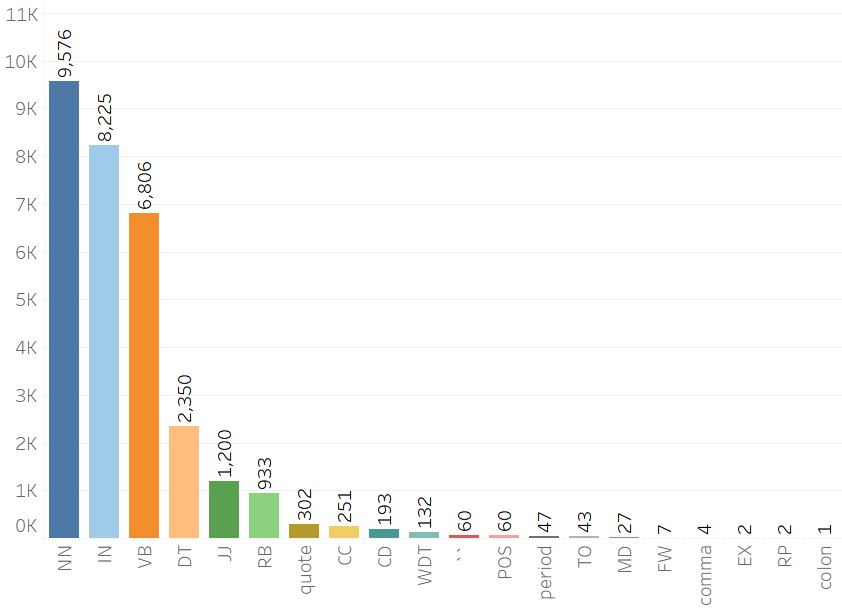
\includegraphics[width=0.95\linewidth]{histogram_2.jpg}
    \vspace{-3mm}
    \caption{ Distribution of POS tags that were assigned the highest attention weights by decomposable attention for incorrectly classified cross-domain examples.}
  \label{fig:attention}
\vspace{-6mm}
\end{figure}



 With this analysis, I was able to confirm that most of the weight is assigned to POS tags of nouns or elements of noun phrases, which confirms my observation that these models anchor themselves on lexical information that is more likely to be domain dependent. 
 As expected, even though this method achieves high accuracy when evaluated in the same domain, the performance in the target domain is poor, marginally above chance.






\subsection{Proposed Delexicalization Techniques}
To mitigate the potential domain dependence introduced by these large attention weights, I propose several semantic masking techniques, which I compare with a deletion baseline.  
Particularly I experiment with several strategies for delexicalization, i.e., where lexical tokens are replaced (or masked) with indicators of their class. While the technique of delexicalization (or masking) has been used before~\citep*{zeman2008cross}, I have expanded it by incorporating semantic information (the assumption that meaning arises from a set of independent and discrete semantic units)~\citep*{peyrard2019simple}. In particular, I first replace named entities with their corresponding semantic tags from Stanford's CoreNLP \citep*{manning2014stanford}. 
To keep track of which entities are referenced betIen claim and evidence sentences, I extend these tags with unique identifiers. Second, I similarly replace other word classes in the sentence (common nouns, verbs, adjectives, and adverbs)  with their super sense tags \citep*{ciaramita2003supersense}.




\subsubsection{Masking Techniques} \label{masking_techniques}
In this section I describe in detail various masking techniques which were used in the experiments. Examples of each form of masking are shown in Table~\ref{masking_examples}.


\begin{table*}[t]
\begin{center}
\begin{tabular}{p{20mm}|p{55mm}|p{70mm}}

\textbf{Config.} & \textbf{Claim}& \textbf{Evidence} \\ \hline
Lexicalized & {With Singapore Airlines, the Airbus A380 entered commercial service.} & {The A380 made its first flight on 27 April 2005 and entered commercial service on 25 October 2007 with Singapore Airlines.}\\
\hline 
NE Deletion & {With  , the  entered commercial service.} & {The A380 made its  flight on  and entered commercial service on  with.}\\
\hline 
Basic NER  & {With \texttt{organization}, the \texttt{miscellaneous} entered commercial service.} & {The A380 made its \texttt{ordinal} flight on \texttt{date} and entered commercial service on \texttt{date} with \texttt{organization}.}\\
\hline 
OA-NER  & {With \texttt{organization-c1}, the \texttt{misc-c1} entered commercial service.} & {The A380 made its \texttt{ordinal-e1} flight on \texttt{ date-e1} and entered commercial service on \texttt{date-e2} with \texttt{organization-c1}.}\\
\hline 

\mbox{OA-NER+SS} Tags & {With \texttt{organization-c1}, the \texttt{artifact-c1} \texttt{motion-c1} commercial \texttt{act-c1} .} & {The A380 \texttt{stative} its \texttt{ordinal-e1 cognition-e1} on \texttt{date-e1} and \texttt{motion-c1} commercial \texttt{act-c1 on date-e4} with \texttt{organization-c1}.  
}\\

\end{tabular}
\end{center}

    \caption{ Example illustratingmy various masking techniques, compared to the original fully lexicalized data. Note that the masking tags were generated with real-world (imperfect) tools. For example, "Airbus A380" in the claim was correctly classified as \texttt{miscellaneous} by the NER tool, while ``A380" in the evidence was not, thus preventing us from taking advantage of the overlap. }
    \label{masking_examples}
\end{table*}


\begin{enumerate}
\item \textbf{Named Entity (NE) Deletion Baseline:}
In this technique the lexical items which are tagged as named or numeric entitiesnamed entities by CoreNLP's named entity recognizer (NER)~\citep*{manning2014stanford} are deleted.  

\item {\flushleft{\textbf{Basic NER:}}}  Token sequences which are labeled as named entities are replaced by the corresponding label, e.g., \texttt{location, person}.

\item {\flushleft{\textbf{Overlap Aware NER (OA-NER)}: }} This technique additionally captures the \textit{lexical overlap} between the claim and evidence sentences with entity ids.  
That is, the first instance of a given entity in the claim is tagged with \texttt{c1}, where the \texttt{c} denotes the fact that it was found in the claim sentence (e.g., \texttt{person-c1}). Wherever this {\em same} entity is found later, in claim or in evidence, it is replaced with this unique tag. If an entity is found only in evidence, then it is denoted by an \texttt{e} tag. (e.g., \texttt{location-e3} would be the third location found only in the evidence).

For example, in the claim-evidence pair shown in Table~\ref{masking_examples}, when the named entity \textit{Singapore Airlines} appears in the claim it is replaced with \texttt{organization-c1}, since it is the first \texttt{organization} to appear in claim. 
The same id is used wherever the same entity is seen again, e.g., in the evidence sentence. However, the date \textit{27 April 2005} occurs only in the evidence, and hence it is replaced with \texttt{date-e1}.
Importantly, I create pseudo-pretrained embeddings for these new OA-NER-based tokens by adding a small amount of random Gaussian noise (mean 0 and variance of 0.1) to pre-trained embeddings~\citep*{pennington2014glove} of the root word corresponding to the category (e.g., \textit{person}). Thus the embeddings of all the sub-tags, while being unique, are close to that of the root word.
\item {\flushleft{\textbf{OA-NER + Super Sense (SS) Tags}}}:
Super-sense tagging is a sequence modeling approach that annotates phrases with coarse WordNet senses~\citep*{ciaramita2003supersense}~\citep*{miller1990introduction}. In this masking method, I not only replace named entities with their OA-NER tags, but also replace other lexical items with their corresponding super sense tags, if found. As with the OA-NER approach, the lexical overlap is also explicitly marked for all these tags with unique ids (see Table~\ref{masking_examples}). 
\end{enumerate}

\begin{table*}[t]
\begin{center}
\begin{tabular}{p{22mm}|p{9mm}p{9mm}p{9mm}p{9mm}}
 & \multicolumn{4}{c}{Configuration} \\
 \hline
Train Domain & {FNC}& {FEVER}  & {FEVER} & {{FNC}} \\ 
Eval Domain & {FNC}& {{FNC}}  & {FEVER} & {{FEVER}} \\ \hline
Masking & & & & \\
\hline
Lexicalized &68.99\%& {48.86\%} &83.43\%& {41.16\%} \\
%\hline
Deletion  &66.45\%& 40.23\% &75.34\%& 33.33\% \\
%\hline
Basic NER &69.40\%& 46.27\% &76.23\%& 35.72\%\\
%\hline 
\textbf{OA-NER} &65.85\%& \textbf{53.59}\% &{82.31\%}& {46.47\%}\\
%\hline 
\textbf{OA-NER+SS} & 45.51\%& 46.71\% &75.26\%& {\bf 51.77\%}\\
\end{tabular}
\end{center}
    \caption{\label{crossdomain} Various masking techniques and their performance accuracies, both in-domain and out-of-domain.} \label{tab:results}

\end{table*}
Since these techniques are general and compatible with most existing semantic representations, I believe they can be further extended onto datasets used for other natural language processing tasks. Thus, by enabling integration of these techniques into the training pipeline, I hope to control lexicalization in the datasets which the neural network methods possibly depend upon. 




\subsection{Results} 
\label{sec:results}


\subsubsection{Phase 1}

In the first phase of experiments, the proposed masking strategies were tested on two fact verification datasets, FEVER and FNC where a decomposable attention model was trained with each of my masking approaches, as well as with the original fully lexicalized input.  Table \ref{tab:results} shows the results of these experiments.
First, I note that indeed the fully lexicalized model, which performs well in-domain, transfers very poorly to a new domain.  
For example, the lexicalized model trained on FEVER,  gave an accuracy of 83.43\% when tested on FEVER, but reduced to 48.86\% when tested on FNC.
This verifies my findings that the signal the model learns from unmasked text does not generalize well.
Additionally, the deletion baseline performs even worse than the fully lexicalized model, which indicates that while the original text can be too domain-specific, its semantic content needs to be maintained on some level. \\
Further, I see that all of my masking approaches improve accuracy in the cross-domain setting, by as much as 10.6\% (25.8\% relative), while still maintaining strong in-domain performance (dropping only a few percentage points).
The best cross-domain performance is obtained using my methods which are overlap-aware, suggesting that even when content is abstracted (i.e., masked), the model benefits from explicit awareness of lexical overlap for fact verification. For example, the overlap-aware SS tagging model that was trained on FNC, gave the highest accuracy of 51.77\% when tested out-of-domain, on FEVER.

I note that the model trained on FNC is able to get optimal performance in the FEVER dataset when using the OA-NER + SS tag masking, while the addition of super sense tags did not benefit the model that was trained on FEVER.  
This could be due to the fact that overall, the evidence provided in FNC is much longer than that of FEVER,
and perhaps the model needs more training data to learn stable signal from the SS tags. 
More importantly, this also suggests that while I have demonstrated that semantic masking is clearly beneficial, it is unclear exactly what level of masking granularity should be employed for a given domain -- from coarse-grained NER tags, to the more granular super sense tags, perhaps even to very fine-grained tags such as those proposed by \citet{ling2012fine}.

\subsubsection {Phase 2}

To further verify these results found in Phase 1, I extend the testing to one more dataset (e.g. MNLI) and by using one more state-of-the-art models (Enhanced Sequential Inference (ESIM)  \cite{chen2016enhanced}). Table~\ref{results} shows the performance of both of the neural network methods (decomposable attention and ESIM) on  both the lexicalized and delexicalized versions of the MNLI dataset. All the methods were re-trained out of the box (without any parameter tuning) and tested on the corresponding evaluation partitions of the dataset. As shown in the table, the accuracies of both the methods remain at par when trained with the delexicalized version of the dataset. 


 
Further to test the effect of delexicalization on domain transferability I pick one of the methods, decomposable attention, train it in one domain and test it in an out-of-domain setting. These results can be seen in Table ~\ref{results_outofdomain}. Specifically, the table shows the accuracies when the model was trained on MNLI and then tested on MedNLI datasets. The results show that the accuracy of the delexicalized model remain at par with that of the model trained on lexicalized model. This aligns with my initial hypothesis that delexicalization helps towards de-biasing these datasets, and thus preventing the neural network methods from being \textit{distracted} by statistical patterns that are not meaningful for the task at hand.

In total the experiments summarized in all these tables highlight three observations: 

\begin {enumerate}
\item The models trained on delexicalized data do not perform worse than the ones trained using lexicalized datasets; 
\item In the two settings with texts where the named entities discussed are well covered by the NER used in this work (from FEVER to FNC, and from FNC to FEVER), the results demonstrate that the semantic lifting provided by my OA-NER method improves domain transfer considerably;  

\item I do not see a significant improvement in the transition from MNLI to MedNLI.  I suspect this is because of the limited overlap of named entity types between the MedNLI and MNLI. For example while the named entity recognizer (CoreNLP) I used, focuses on PERSON, ORGANIZATION, etc. the MedNLI dataset contains more medical terms related diseases and symptoms. This possibly necessitates the importance of exploring using a domain-relevant NER.

\end {enumerate}



\begin{table*}[t]
\begin{center}
\begin{tabular}{|p{20mm}|p{20mm}|p{20mm}|p{20mm}|p{20mm}|p{20mm}|p{20mm}|}
\hline 
\textbf{Method} & \textbf{MNLI matched lexicalized }& \textbf{MNLI matched delexicalized } & \textbf{MNLI mismatched lexicalized } &\textbf{MNLI mismatched delexicalized } \\
 \hline
decomposable attention & {60.95\%} &{64.52\%} &{61.43\%}&{64.86\%}\\
\hline 
ESIM  & {68.84\%} &{68.14\%} &{69.40\%}&{69.10\%}\\
\hline 
\end{tabular}
\end{center}
\caption{Performance of various high performing neural network methods over lexicalized and delexicalized versions of the same dataset. `Matched' is the in-domain partition of the MNLI validation dataset, and `mis-matched' is the out-of-domain partition. The performance of both the methods remain close to each other in delexicalized and lexicalized versions of the same dataset, which validates that my  delexicalization techniques preserve the original information of the text. }

    \label{results}
\end{table*}



\begin{table*}[h]
\begin{center}
\begin{tabular}{|p{25mm}|p{12mm}|p{11mm}|p{10mm}|}
 \hline
\textbf{Train Domain} & \textbf{MNLI} \\ 
 \textbf{Eval Domain} & \textbf{MedNLI} \\ 
\hline
Lexicalized &51.47\% \\
OA-NER &51.57\%\\
\hline
\end{tabular}
\end{center}
    \caption{ Performance accuracies of the Decomposable Attention against various masking techniques when tested out-of-domain. The ``Train Domain'' row indicates the training datasets, while the ``Eval Domain'' indicates the domain of the corresponding evaluation partitions. For example, one experiment trained the decomposable attention method on FEVER and evaluated the resulting model on the testing partition of FNC (column 3). }
    
    \label{results_outofdomain}
\end{table*}


\begin{table*}[h!]
\begin{center}
\begin{tabular}{|p{20mm}|p{9mm}|p{10mm}|}
 \hline
\textbf{Masking strategy} & \textbf{FNC}  & \textbf{FEVER}  \\ 
\hline
Lexicalized &68.99\% &83.43\% \\
OA-NER &65.85\% &82.31\%\\
OA-NER+SS & 45.51\% &75.26\%\\
\hline
\end{tabular}
\end{center}
    \caption{Performance accuracies of the Decomposable Attention against various masking techniques when tested in-domain for FNC and FEVER datasets. The ``Lexicalized" row shows the accuracies when decomposable attention was trained using the corresponding lexicalized data. This demonstrates that while delexicalization with OA-NER maintains the performance, the addition of Super Sense tags reduces the accuracy, emphasizing the fact that the amount of granularity to use is still an open problem.}
    \label{sstag}
\end{table*}


Also this work touches upon questions about which granularity offers a good approximation of semantic meanings. For example, Table ~\ref{sstag} shows the performance of Decomposable Attention against various delexicalization strategies. It can be seen that, while the addition of OA-NER tags does not change the performance significantly, the semantic lifting provided by the SS tags decreased the accuracies considerably in both cases (FEVER and FNC).  This demonstrates that while generalizing away from lexical items is important, {\em how much} to generalize remains an open research problem. One future direction of interest is exploring the right level of masking granularity needed for delexicalization, which is likely dependent on the task. 



These results, which were published as \citep*{emnlp2019sandeep}, demonstrate that my masking strategy is successful in mitigating the dependency on domain-specific lexical information and aids in certain domain transfer transitions. 

 
\section{Future Work/Plan for Dissertation}
In the previous sections I investigate the need for delexicalization techniques to reduce the potential dependence of neural network methods on lexicalized items in natural language inference tasks. My experiments show that delexicalization achieves comparative results {\em in-domain} with the state of the art methods trained on lexicalized data. Importantly, I show that methods trained on delexicalized data transfer considerably better {\em out-of-domain}, which  confirms the importance of delexicalization in natural language inference tasks for domain transferability.

In this section I describe a few proposed solutions where I explore combining delexicalization with knowledge distillation to transfer learning across domains.





\subsection{Knowledge Distillation of Data}
Knowledge distillation is a training procedure where one neural network method functions as a \textit{teacher} and transfers its knowledge to a \textit{student} model. While the intuition for knowledge distillation was suggested in \citep*{ba2014deep} it was formally introduced in \citep*{hinton2015distilling}. The motivation behind knowledge distillation is to reduce computation complexity of deep neural network architectures to smaller ones. This facilitates the deployment of such architectures in memory constrained devices. The intuition behind knowledge distillation is that a given deep learning model, when it learns to discriminate between a large number of classes, also assigns probabilities to incorrect answers, which are often overlooked. While these probabilities are small for a given incorrect class (and hence not chosen as the right answer for that data point), some of these probabilities are much larger than those assigned to some other incorrect classes. These relative probabilities of incorrect answers are then used  to learn about how the model tends to generalize. So when knowledge is distilled from a large model into a smaller one, the smaller model can be trained to generalize in the same way as the large model. The assumption is that if the larger model generalizes well, a smaller model trained to generalize in the same way will do better when compared to another small model that was trained on much lesser data than the original large model. To enable this transfer the knowledge distillation models (also known as teacher student models) use the class probabilities of the larger model (frequently referred to as \textit{soft targets}) to train the smaller model. Further, when the larger model consists of an ensemble of models, an arithmetic mean or geometric mean of their individual predictive distributions are used as soft targets. In many knowledge distillation architectures the logits (inputs to the final sotmax) rather than the probabilities produced by the softmax (the correct answers) are the targets for learning the small model. The optimization is then typically achieved by minimizing the squared difference (as opposed to maximizing the average log probability of correct answers that a stand alone model would have used) between the logits of the larger and smaller models. The aim thus of distillation architectures is to \textbf{\textit{raise the temperature}} of the final softmax until the larger model produces a suitably soft set of targets. Then the same \textit{high temperature} is used to train the smaller model to match these soft targets. Typically, while the datasets used to train both the larger and smaller models are the training data itself, there are variations where smaller model is trained on an unlabeled version of the same training data (i.e.,unsupervised training).


\subsection{Related Work}


Many previous methods using knowledge distillation focus on task-specific knowledge distillation, which transfers knowledge from a single-task teacher to its student. Tzeng et al.\citep*{tzeng2015simultaneous}, use data distillation in a visual domain adaptation setting in order to transfer class correlations between domains. 

Papernot et al. \citep*{papernot2016distillation} use distillation as a defense to adversarial perturbations against deep neural networks. More recently in Sun et al. \citep*{sun2019patient} , Jiao et al. \citep*{jiao2019tinybert},  Zhao et al.\citep*{zhao2019extreme}, and Tang et al. \citep*{tang2019distilling} the knowledge distillation algorithms are specially designed for transformer-based architectures, and the student models are adapted from teacher models. Liu et al. \citep*{liu2019attentive}, explore the knowledge distillation method under the setting of multi-task learning \citep*{caruana1997multitask} \citep*{baxter2000model}.




\subsection{Proposed Solution}

Most of the research so far in knowledge distillation has thus been about transferring the form of model while keeping the same knowledge. In this work I propose to use the same data distillation framework, but aim to keep the model stable and transfer the underlying data semantics instead. This proposal is based on the assumption that a more abstract view of the knowledge contained in a dataset, once freed from particular instantiations related to a given domain, can be used to transfer learning across domains. I propose to distill the student model from one or more teachers where the teacher model will be trained on the lexicalized version of a given dataset, while the student model will be trained from the corresponding delexicalized version (refer masking/delexicalization techniques mentioned above) of the same dataset. The reasons for this setup are as follows:

\begin{itemize}
  \item The distilled model learns a more universal language representation by leveraging the cross-lexicalized-delexicalized data.
  \item The student model will achieve comparable accuracy in an in-domain setting.
  \item Since the proposed framework is quite general, where the data of the student model is independent of the teacher model, this possibly can enable the transfer of knowledge across domains.
\end{itemize}

Motivated by the above reasons, I plan to apply knowledge distillation towards solving the domain- transfer problem mentioned above. This is inspired from the idea that datasets in similar domains are possibly related by means of a common low dimensional semantic representation. I propose that using the shared structure within a student teacher model could possibly help by assuming some connections over the underlying data distribution of different datasets. Although many of the recent knowledge distillation works \citep*{jiao2019tinybert,tang2019distilling,zhao2019extreme}  employ a  pretrained language model as the underlying neural network architecture, I plan to choose simple attention based models adapted from ~\citep*{parikh2016decomposable} and \citep*{chen2016enhanced}. The reasons are:

\begin{itemize}
  \item Both these models have been proven to achieve state of the art results in natural language inference related tasks especially due to their inherent attention mechanisms.
  \item My approach is more data driven and hence simpler transparent models will enable me to focus on the important semantic transitions needed (e.g.,choice of different masking methods) and their influence in transferring knowledge across domains.
 \end{itemize}



\section{Conclusion}

 In this work I investigate the need for delexicalization techniques to reduce the potential dependence of NN methods on lexicalized items in NLI tasks. I specifically explore two masking techniques to delexicalize datasets: the first one replaces the lexical entities in an overlap-aware manner, and the second one additionally incorporates semantic lifting of nouns and verbs. My experiments show that delexicalization achieves comparative results {\em in-domain} with the state of the art methods trained on lexicalized data. Importantly, I show that methods trained on delexicalized data transfer considerably better {\em out-of-domain}, which  confirms the importance of delexicalization in NLI tasks for domain transferability. 
 
Next I suggest my plans to explore combining delexicalization with knowledge distillation to transfer learning across domains. Specifically, here  I propose a new variant of the data distillation student teacher framework for learning underlying data semantics to enable domain transfer. Instead of transferring knowledge between different architectures I propose to use the knowledge extracted from a lexicalized dataset in improving a deep neural network which by itself also learns from the corresponding delexicalized dataset. To the best of my knowledge, my proposed method is novel and hence I hope it to contribute significantly to my PhD Dissertation.




\balance
\begin{spacing}{0.88}
\bibliographystyle{unsrtnat}
\bibliography{compre_masking}
\end{spacing}

% that's all folks
\end{document}